\section{Scanner and Parser Generators}
\begin{frame}{Scanner and Parser Generators}
  \begin{itemize}
    \item Parser overview
    \item Parser generators
    \item Lexer
    \item CFG
  \end{itemize}
\end{frame}

\begin{frame}{Parser overview}
  Automate the generation of lexer and parser.
\begin{figure}[ht]
\centering
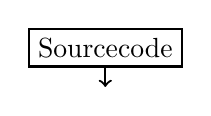
\begin{tikzpicture}
  \draw [thick, ->] (0,0.3) -- (0,0);
  \node [rectangle, draw, thick,fill=white!20] at (0,0.5) {Sourcecode};
\end{tikzpicture}

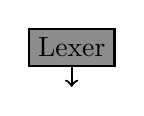
\begin{tikzpicture}
  \draw [thick, ->] (0,0.3) -- (0,0);
  \node [rectangle, draw, thick,fill=gray!90] at (0,0.5) {Lexer};
\end{tikzpicture}

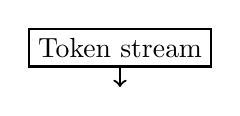
\begin{tikzpicture}
  \draw [thick, ->] (0,0.3) -- (0,0);
  \node [rectangle, draw, thick,fill=white!20] at (0,0.5) {Token stream};
\end{tikzpicture}

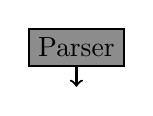
\begin{tikzpicture}
  \draw [thick, ->] (0,0.3) -- (0,0);
  \node [rectangle, draw, thick,fill=gray!90] at (0,0.5) {Parser};
\end{tikzpicture}

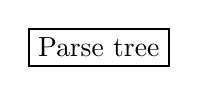
\begin{tikzpicture}
  \node [rectangle, draw, thick,fill=white!20] at (0,0.5) {Parse tree};
\end{tikzpicture}
\end{figure}
\end{frame}

\subsection{Parser Generators}
\begin{frame}{Parser Generators}
  \framesubtitle{Different parser generators}
  \begin{itemize}
    \item SableCC
    \item JavaCup
    \item ANTLR
    \item Coco/R
    \item Yacc
    \item And many mores.
  \end{itemize}
\end{frame}

\begin{frame}{SableCC}
  \begin{itemize}
    \item An Item
  \end{itemize}
\end{frame}

\begin{frame}{JavaCup}
  \begin{itemize}
    \item An Item
  \end{itemize}
\end{frame}

\begin{frame}{ANTLR}
  \begin{itemize}
    \item An Item
  \end{itemize}
\end{frame}

\subsection{Tokens and Lexer}
\begin{frame}{Tokens}
  \begin{itemize}
    \item TOKENS!
  \end{itemize}
\end{frame}

\begin{frame}{Lexer}

\end{frame}


\subsection{CFG}
\begin{frame}{GAMBL's CFG}

\end{frame}

\begin{frame}{Alternative CFG}

\end{frame}

%JUST FOR PUNS